\documentclass[a4paper,10pt]{article}

% Hier die Nummer des Blatts und Autoren angeben.
\newcommand{\blatt}{8}
\newcommand{\autor}{Ralf Engelken, Joachim Schmidberger, Frank Woithe, Michael Steinke, Merlin Koglin}

\usepackage{hci}


\begin{document}
% Seitenkopf mit Informationen
\kopf
\renewcommand{\figurename}{Figure}

\aufgabe{13 \textit{(Team-Aufgabe)}} 
Wählen Sie aus den folgenden Anwendungsdomänen jeweils ein konkretes interaktives System aus und beschreiben Sie das Konzeptionelle Modell dahinter. Konkretisieren Sie dies, indem Sie mindestens drei Interface-Elemente (pro System) auswählen und die dahinter stehende Metapher erklären. \newline
 
\textbf{\textit{1. eCommerce/Web-Shop (z.B. Amazon, Zalando, ...)}} \newline

LORUM IPSUM ... \newline

\textbf{\textit{2. Mediaplayer (um Audio oder Video Dateien abzuspielen)}} \newline

LORUM IPSUM ... \newline

\textbf{\textit{3. soziales Netzwerk}} \newline

Soziale Netzwerke versuchen konzeptionell kommunikationsbereiche eines Menschen in einem Netzwerk abzubilden. Dabei bedienen Sie sich an der "öffentlichkeit" der Kommunikation, also ob diese
\begin{enumerate}
\item zwischen zwei oder mehreren bekannten Menschen (z.B. Gruppennachrichten die eine direkte Konversation nachbilden können)
\item in einer offenen oder geschlossenen Gruppe, in der sich nicht jeder kennt oder(Forum oder Gruppen, die eine Konversation in einem Verein nachbilden können)
\item ungerichtet und dabei zwischen dem Individuum und allen bekannten und unbekannten (z.B. eine Nachricht an unbekannte über einen Zettel an der Staße (Suche Wohnung ect. pp))
\end{enumerate}

stattfindet. \newline

Ein Beispiel für ein soziales Netzwerk ist \textbf{\textit Facebook}, welches jedoch noch mehr Konzepte auf seiner Plattform mit dem kommunikations-Konzept verknüpft. Im Folgenden soll es nur um die Kommunikation gehen.

\begin{figure}[ht]
\centering 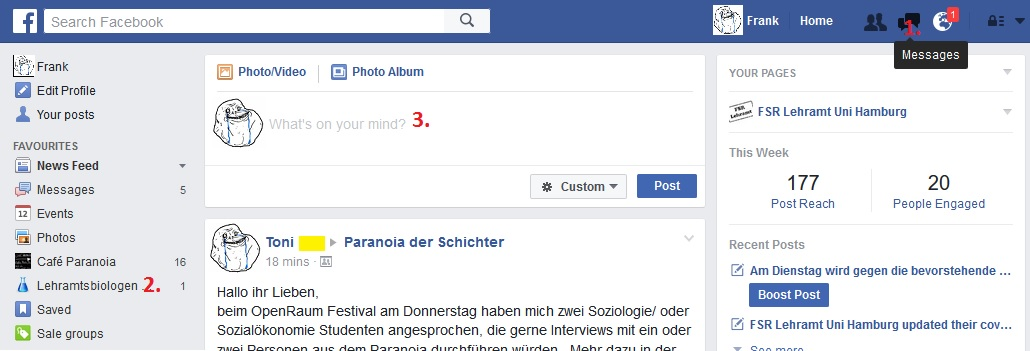
\includegraphics[width=1\textwidth]{facebook.jpg}
\caption{Navigations-Metaphern auf Facebook: 1. Nachrichten, 2. Symbol für eine (geschlossene) Gruppe, 3. die Pinnwand mit den Öffentlichkeitseinstellungen}
\end{figure}

Das Nachrichtensymbol (1) besteht aus zwei ineinander verschachtelten Sprechblasen. Sprechblasen werden oft als graphisches Mittel eingesetzt, um Gespräche zu symbolisieren. Das Symbol ist also eine Methaper für ein Gespräch zwischen zwei oder mehreren Personen. \newline
Die Metapher für eine Gruppe, in dem Fall die Gruppe 'Lehramtsbiologen' (2), besteht aus einem Reagenzglas und dem Text. An einem passenden Icon und dem Text soll der User erkennen um welche Art von Gruppe es sich handelt und auf dieses Klicken um den den Inhalt der Gruppe anzuzeigen. Fährt der User mit der Maus über die Gruppe, so wird sie etwas grauer hinterlegt, was einen Link oder klickbares Element andeutet. \newline
Die Pinnwand (3) trägt den Namen der Methapher schon in sich, denn sie soll wie eine Pinnwand im richtigen Leben fungieren. Je nachdem wo diese Pinnwand hängt (z.B. in einem abgeschlossenem Raum oder sichtbar zur Straße hin) sehen mehr oder weniger Menschen eine Nachricht auf dieser. Gleiches gilt auch hier: Der user schreibt eine Nachricht auf seine Pinnwand und "postet" diese. Über den Button "Custom" kann er noch einstellen, wer diese Nachricht sehen kann. \newline


\textbf{\textit{4. ein Programm/Website aus einer beliebigen weiteren Anwendungsdomäne}} \newline

LORUM IPSUM ... \newline


\end{document}
